\documentclass[12pt]{article}

\usepackage{sbc-template}
\usepackage{graphicx,url}
\usepackage[utf8]{inputenc}
\usepackage[brazil]{babel}
\usepackage{listings}
\usepackage[normalem]{ulem}
\useunder{\uline}{\ul}{}
\usepackage{longtable}
\usepackage[justification=centering]{caption}
\usepackage{float}

\lstset{
	numbers=left,
	stepnumber=1,
	firstnumber=1,
	numberstyle=\tiny,
	extendedchars=true,
	breaklines=true,
	frame=single,
	showstringspaces=false,
	xleftmargin=2.5em,
	framexleftmargin=2em,
	basicstyle=\small,
}

\renewcommand{\lstlistingname}{Código}
\renewcommand{\lstlistlistingname}{Lista de Códigos}

     
\sloppy

\title{Planejamento de um Experimento sobre uso de Diretrizes de \textit{Design} e Compreensão da Informação em um Aplicativo de Ensino sobre Infecções Sexualmente Transmissíveis}

\author{Diogo C. T. Batista\inst{1}, Elissandra G. Pereira\inst{1}}

\address{Universidade Federal do Paraná (UFPR)\\
	Curitiba -- Paraná -- Brasil
	\email{diogocezar@ufpr.br,egpereira@inf.ufpr.br}
	}

\begin{document}

\maketitle

\begin{resumo}
	Este projeto descreve o planejamento de um experimento de validação do uso de diretrizes de \textit{design} no auxílio da compreensão da informação em um aplicativo de ensino sobre infecções sexualmente transmissíveis. O alvo do estudo é orientado à exposição de duas opções do mesmo conteúdo, na primeira expõe-se apenas um texto original com os conteúdos sobre as doenças, na segunda, apresenta o mesmo conteúdo com redesign seguindo diretrizes de \textit{design}. Para análise dos resultados, definiu-se a execução de um questionário que avalia a compreensão do conteúdo.
\end{resumo}

\section{Definição do Objetivo}

De acordo com o paradigma GQM, os objetivos deste experimento podem ser definidos como:

\begin{itemize}
	\item \textbf{ANALISAR}: Uso de diretrizes de \textit{design} para material educativo digital;
	\item \textbf{COM O PROPÓSITO DE}: Avaliar;
	\item \textbf{COM RESPEITO A}: Compreensão do conteúdo;
	\item \textbf{NO PONTO DE VISTA}: Dos pesquisadores do projeto;
	\item \textbf{NO CONTEXTO DE}: Alunos universitários avaliando a compreensão do conteúdo das duas versões do protótipo.
\end{itemize}

\section{Formulação de Hipóteses}

Propõe-se a utilização de hipóteses do tipo \textit{nula} e \textit{alternativa}, sendo:

\begin{itemize}
	\item \textbf{Hipótese Nula - H0}: Não há diferença entre a compreensão do conteúdo na versão do protótipo do aplicativo sem uso das \textit{guidelines} de \textit{design} em relação a versão com o uso das \textit{guidelines};
	\item \textbf{Hipótese Alternativa - H1}: Há diferença entre a compreensão do conteúdo na versão do protótipo do aplicativo sem uso das \textit{guidelines} de \textit{design} em relação a versão com o uso das \textit{guidelines}.
\end{itemize}

\section{Seleção de Variáveis}

Utiliza-se a seleção de variáveis \textit{dependentes} e \textit{independentes}:

\begin{itemize}
	\item \textbf{Variáveis Independentes}: protótipos do aplicativo (original ou com \textit{guidelines} aplicadas); 
	\item \textbf{Variáveis dependentes}: compreensão do conteúdo, satisfação do usuário ao pesquisar o conteúdo, satisfação do usuário com a aparência da tela.
\end{itemize}

\subsection{Definição da coleta e cálculo das variáveis dependentes}

A coleta das variáveis dependentes se fará através de um questionário. O questionário será composto de perguntas relacionadas a compreensão do conteúdo e satisfação do usuário. Na compreensão do conteúdo, será calculada a quantidade de pessoas que acertaram questões sobre o conteúdo. Na satisfação, será considerada a quantidade de pessoas que gostaram da diagramação do conteúdo e o grau de dificuldade que tiveram em encontrar as informações, ambos medidos através de uma escala Likert.

\section{Especificação do \textit{design} do estudo}

O experimento será realizado em um formato \textit{between group}. Com essa estratégia, os participantes serão divididos em dois grupos. Cada grupo será exposto a uma versão diferente do aplicativo. Com issom garante-se a maior imparcialidade no experimento, visto que em uma outra possível abordagem, do tipo \textit{within group}, que definiria que cada participante seria exposto a ambas versões, o usuário poderia aprender com uma versão do aplicativo, tendo maior facilidade na avaliação da segunda versão fosse realizar o teste.

Na utilização da estratégia \textit{between group}, os grupos foram divididos para usar cada um uma versão de um protótipo de app baseado em diretrizes. As diretrizes são listadas a seguir.

\subsection{Lista de Diretrizes}

A definição das diretrizes foi baseada no artigo de \cite{JIN2013248}, no qual, argumenta-se que para que para um bom \textit{design} para ensino digital, pode-se ajustar o conteúdo utilizando uma série de diretrizes.

Utilizou-se para o projeto a prototipação de uma tela chamada ``Conhecendo as ISTs'' a prototipagem tanto da réplica da tela original, quanto da tela revisada com as diretrizes foi feita pelo programa Figma.

Das diretrizes propostas por \cite{JIN2013248}, foram selecionadas três para serem aplicadas no redesign da tela, deixando de fora aquelas que exigiam um conjunto de telas, aquelas que necessitavam de ferramentas de animação que o programa utilizado para prototipagem não disponibiliza e aquelas que já foram usadas na tela original do aplicativo.

\subsection{Diretrizes selecionadas}

\subsubsection{A primeira diretriz selecionada}

\begin{quote}
	Use space to separate the paragraphs, subsections, and chapters from one another (Hartley, 1985)
\end{quote}

\begin{figure}[H]
  \centering
  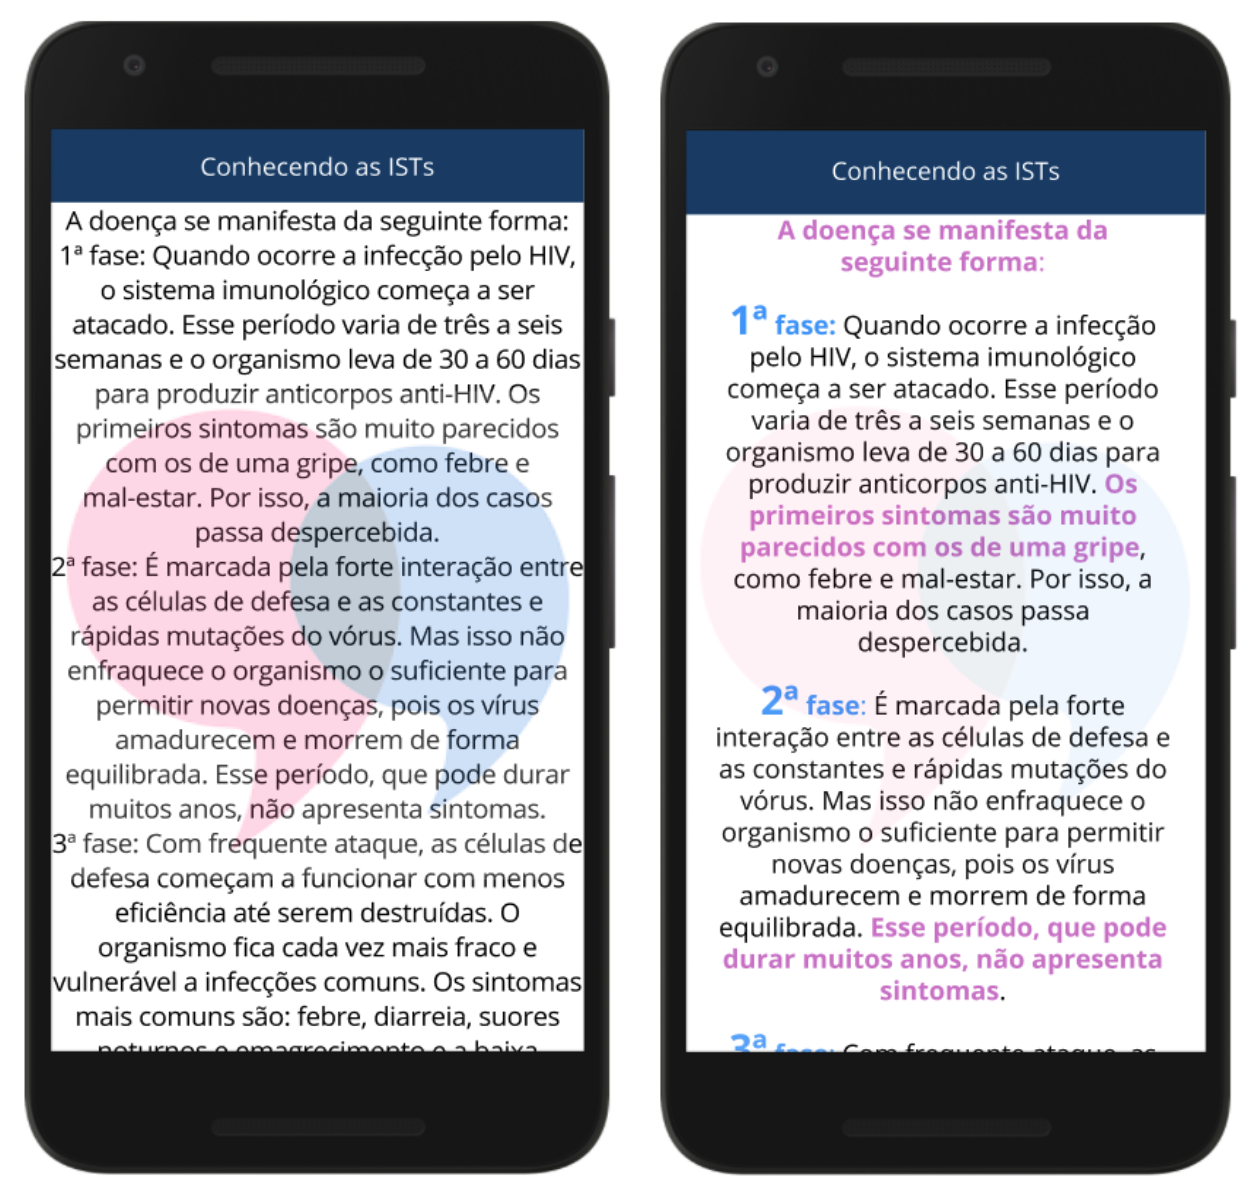
\includegraphics[width=30em]{images/image_1.png}
  \caption{Exemplo de utilização da primeira diretriz}
  \label{fig:img1}
\end{figure}

É possível notar na Imagem \ref{fig:img1}, a tela sem espaço para separação dos parágrafos e sessões (original, à esquerda) e com o espaçamento aplicado (revisada, à direita).

\subsubsection{A segunda diretriz selecionada}

\begin{quote}
	Use color to help users understand what does and does not go together (Leavitt \& Shneiderman, 2006)
\end{quote}

\begin{figure}[H]
  \centering
  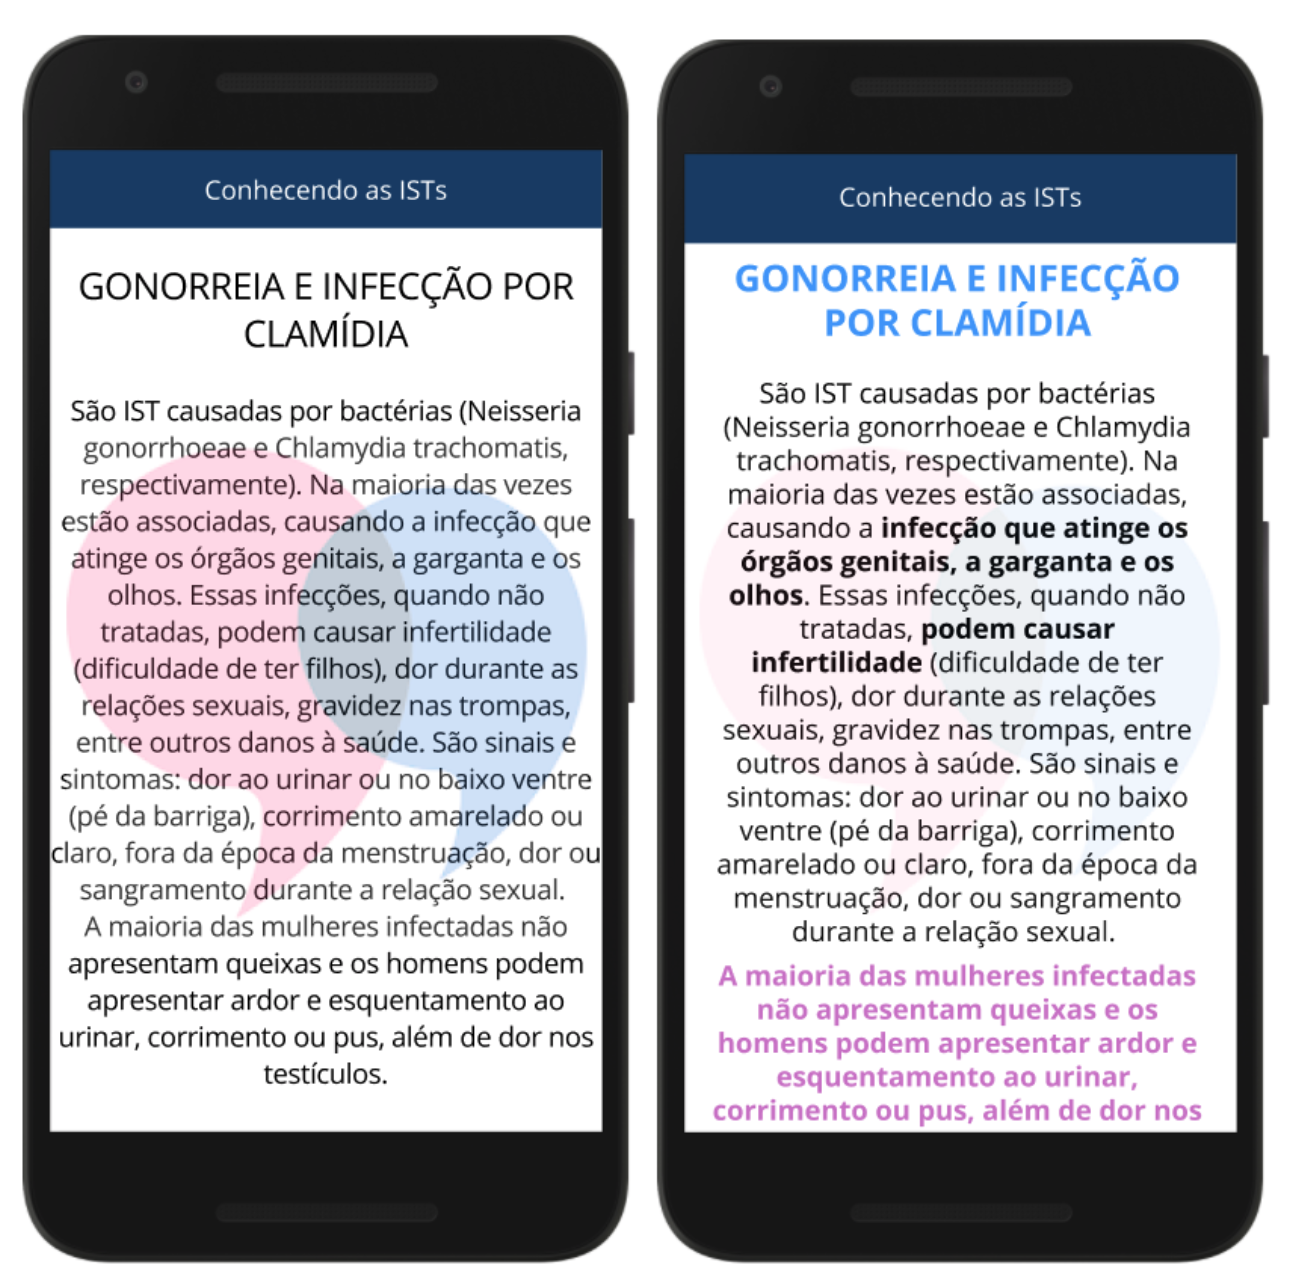
\includegraphics[width=30em]{images/image_2.png}
  \caption{Exemplo de utilização da segunda diretriz}
  \label{fig:img2}
\end{figure}

É possível notar na Imagem \ref{fig:img2}, a tela sem uso de cor (original, à esquerda) e com uso de cor (revisada, à direita).

Foram utilizadas as cores preto, azul e rosa. A maior parte do texto foi mantida em preto, cor original, para permanecer a maior fidelidade ao \textit{design} original do aplicativo e evitar excesso de interferências na hora de testar as diretrizes. As cores adicionais, azul e rosa, seguem a identidade gráfica existente do aplicativo.

\begin{itemize}
\item \textbf{Azul}: Usado para marcar os títulos/palavras chave e avisos de grande importância.
\item \textbf{Rosa}: Usado para destacar os sintomas.
\end{itemize}

\subsubsection{A terceira diretriz selecionada}

\begin{quote}
	Design summary pages at the end of e-learning lessons (Alessi \& Trollip, 2001)
\end{quote}

\begin{figure}[H]
  \centering
  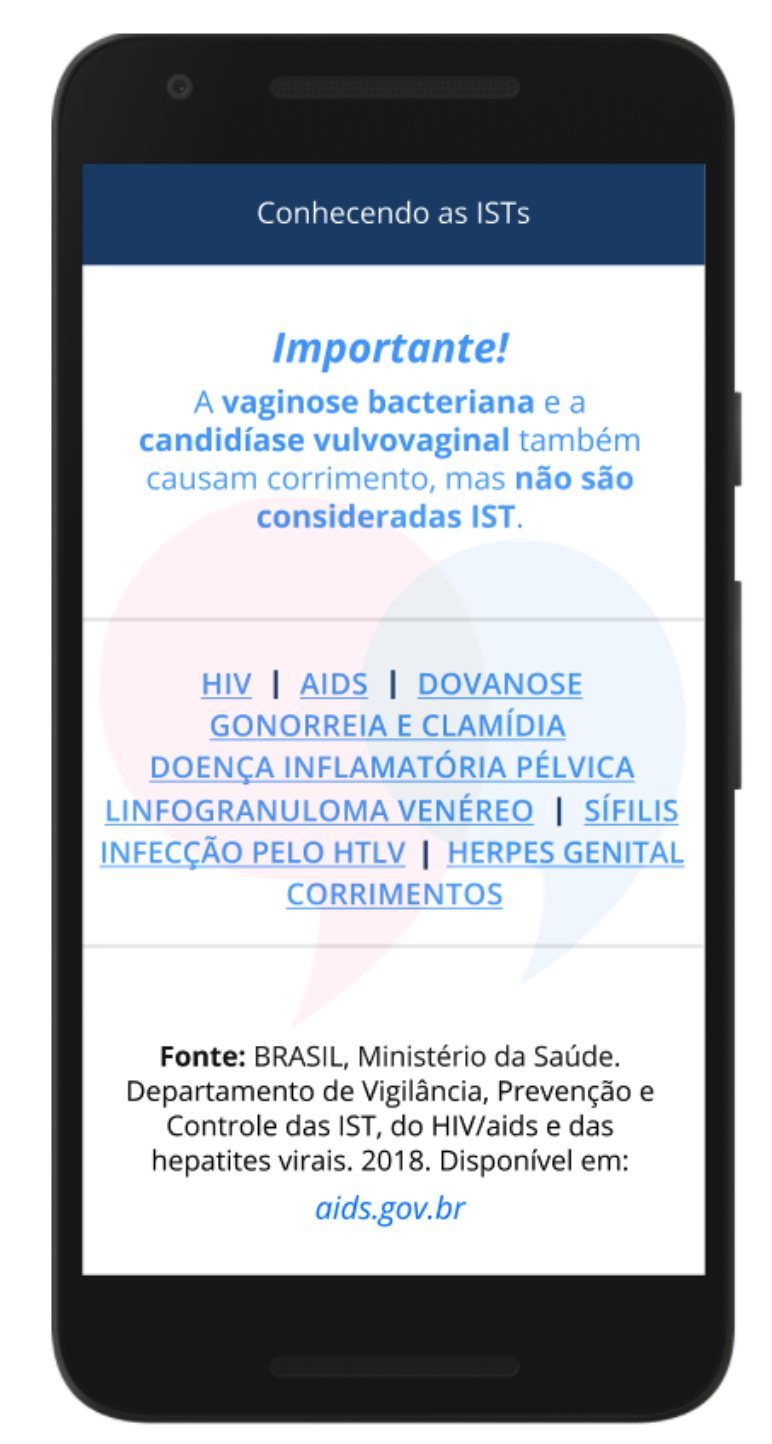
\includegraphics[width=15em]{images/image_3.png}
  \caption{Exemplo de utilização da terceira diretriz}
  \label{fig:img3}
\end{figure}

Nota-se na Imagem \ref{fig:img3}, o resumo das palavras-chave/títulos ao final da tela.

Foram selecionados os títulos de cada doença como palavras-chave para resumir o conteúdo ao final da tela. Adicionou-se também a possibilidade de clicar na palavra e rolar automaticamente para posição da tela em que o conteúdo referente a palavra-chave aparece.

\section{Seleção de participantes e ambiente/local onde o estudo deve ser realizado}

Os participantes foram escolhidos por conveniência e convidados diretamente pelos pesquisadores por email ou aplicativos de mensagens instantâneas. Foram escolhidos como amostra seis estudantes universitários. Apesar de ser homogêneo, o público possui um grau de estudo elevado, além de em sua maioria pertencerem a uma faixa etária entre (23-24 anos) que geralmente possuem domínio de tecnologia, caso este público encontre dificuldades com o sistema, isso impactará que usuários mais leigos possivelmente encontrarão problemas também. 

É importante ressaltar contudo que o oposto não se faz realidade: uma facilidade desse público não necessariamente reflete na facilidade de outros públicos.

Devido às limitações da quarentena, o estudo foi completamente virtual, não necessitando de um ambiente específico para sua realização. O ambiente do estudo se constituiu principalmente do ambiente \textit{desktop} pessoal do participante (foi recomendado aos participantes que o estudo ocorresse no \textit{desktop}). O ambiente \textit{desktop} deveria ser composto de um navegador de internet para acesso de: i) uma versão do protótipo do app e ii) ao formulário online.

\section{Definição de Instrumentação}

O formulário enviado pelo google forms é um instrumento de pesquisa, composto pelo Termo de Consentimento Livre Esclarecido, mais o questionário sobre o conteúdo do aplicativo, assim como as questões de avaliação e de análise de formação e idade dos participantes.

O Termo e o questionário foram enviados aos participantes por meio de um formulário do google. Foram montados dois formulários diferentes, diferindo apenas o link do protótipo. Em um formulário é apresentado um protótipo que replica a tela original, e no outro um protótipo adaptado com as diretrizes. Metade do grupo recebeu um formulário, a outra metade o outro.

O termo de Consentimento Livre e Esclarecido tem como função explicar o motivo do experimento para o participante, assim como seus direitos de pedir ajuda, parar e remover sua participação quando quiser, e avisar que os dados serão anônimos e utilizados para fins acadêmicos.

O questionário foi dividido em quatro sessões, com um total de treze perguntas.

A primeira sessão apresenta o link para o protótipo e as instruções para abri-lo e se familiarizar com o conteúdo. A segunda sessão tem três perguntas sobre o conteúdo do aplicativo, com resposta aberta e obrigatória, cada uma dessas perguntas é diretamente seguida por uma questão de ``sim ou não'' indagando se o participante consultou novamente o material para responder. 

A terceira parte, sobre usabilidade e satisfação, tem duas questões sobre a percepção individual do participante sobre o aplicativo, medidas por escalas Likert, e outras duas questões sobre o que os participantes pensam que outros universitários achariam do aplicativo, com respostas de ``sim ou não''. 

Na quarta e última sessão, foram feitas três perguntas, uma delas sobre o grau de formação universitária (graduação, mestrado ou doutorado, completos ou incompletos), uma pergunta sobre a área do conhecimento (exatas, humanas ou biológicas) e uma pergunta sobre faixa etária.

\section{Avaliação das ameaças à validade}

Neste experimento, considerou-se quatro principais ameaças à validade: 

Validade de conclusão (tamanho da amostra e homogeneidade). O número pequeno de participantes não é desejável para um resultado estatístico. O tamanho da amostra é um problema comum em estudos de IHC. Outra ameaça é a homogeneidade da amostra, visto que todos são estudantes universitários. Para contornar isso, foram convidados participantes de diferentes universidades, áreas do conhecimento e graus de formação universitária.

Ameaça à validade pelo conhecimento prévio dos participantes. Consideramos que os participantes podem ter informações pré concebidas sobre o assunto do aplicativo, podendo gerar uma falha na hora de analisar a compreensão do conteúdo. Para contornar esse viés, instruímos o participante a responder com base apenas aquilo que leu na tela do aplicativo.

Falta de controle do ambiente de teste. Como o experimento foi feito de maneira virtual, é impossível garantir condições iguais de ambiente entre todos os participantes, visto que os mesmos responderam o formulário de suas próprias casas ou local onde se encontravam. Para amenizar esta ameaça foi pedido que os participantes respondessem de maneira individual e isolada, utilizando um dispositivo \textit{desktop}.

\bibliographystyle{sbc}
\bibliography{sbc-template}

\end{document}
